\documentclass[11pt, letter, answers]{exam}
\usepackage[inner=1.5cm,outer=1.5cm,top=2.5cm,bottom=2.5cm]{geometry}
\usepackage{array, booktabs, graphicx, color}
\usepackage{xcolor, enumitem, lastpage}
\usepackage{multirow, multicol, makecell}
\usepackage{amsmath, amssymb, pifont}
\usepackage{float}
\usepackage{parskip}
\usepackage{enumitem}
\usepackage{ifthen}
\usepackage{lipsum}
\usepackage{wasysym}

\usepackage{listings}
\usepackage{xcolor}
\lstset{
    language=Python,
    basicstyle=\ttfamily,
    keywordstyle=\color{blue},
    stringstyle=\color{orange},
    commentstyle=\color{green!50!black},
    breaklines=true,
    showstringspaces=false,
    tabsize=4
}

\usepackage[style=apa]{biblatex}
\bibliography{Slides/references}


%--------------------------------------------------------------
% Header
%--------------------------------------------------------------
\firstpageheader{94-867/19-867/12-768\quad Fall 2026}{}{Carnegie Mellon University}
\runningheader  {94-867/19-867/12-768\quad Fall 2026}{}{Carnegie Mellon University}

\firstpageheadrule
\runningheadrule

%--------------------------------------------------------------
% Footer
%--------------------------------------------------------------
\firstpagefooter{}{}{Page \thepage\ of \pageref{LastPage}}
\runningfooter {}{}{Page \thepage\ of \pageref{LastPage}}

%--------------------------------------------------------------
% Hyperlink setting
%--------------------------------------------------------------
\usepackage{hyperref}
\usepackage{nameref}
\hypersetup{colorlinks=true, linkcolor=blue, urlcolor=cyan, filecolor=magenta}
\sloppy

%--------------------------------------------------------------
% Define grade and solution
%--------------------------------------------------------------
\newcommand{\grade}[1]{
    \small\textcolor{magenta}{\emph{(#1 \ifnum#1=1 point\else points\fi)}}%
    \normalsize
}
\newcommand{\pt}[1]{
    \small{(#1 \ifnum#1=1 pt\else pts\fi)}
    \normalsize
}
\newcommand{\sol}[1]{\ifshowsolutions{\leavevmode{\color{blue}Solution: #1}}\fi}

%--------------------------------------------------------------
% Define question types
%--------------------------------------------------------------
\newcommand{\sOne}{\textbf{Select one: }}
\newcommand{\sAll}{\textbf{Select all that apply: }}
\newcommand{\tof}{\textbf{True or False: }}
\newcommand{\saq}{\textbf{Short answer: }}
\newcommand{\sCode}{\textbf{Show your code: }}
\newcommand{\sPlot}{\textbf{Show your plot: }}
\newcommand{\sCal}{\textbf{Show your calculation: }}

%--------------------------------------------------------------
% Define MCQ options
%--------------------------------------------------------------
\usepackage{tikz}
\usepackage{cancel}
\CorrectChoiceEmphasis{}
\checkedchar{\blackcircle}
\newcommand{\blackcircle}{\tikz\draw[black,fill=black] (0,0) circle (1ex);}

%--------------------------------------------------------------
% Define SAQ answer box
%--------------------------------------------------------------
\usepackage[many]{tcolorbox}
\tcbuselibrary{listings, breakable}
\newtcolorbox{answerBox}[1][]
{
    fit,
    enhanced,
    colback=white,
    sidebyside align=top,
    box align=top,
    #1
}
\newtcblisting{codeBox}[1][]{
    listing only,
    listing options={language=Python, basicstyle=\ttfamily\small},
    top=0pt,
    colback=white,
    enhanced,
    sidebyside align=top,
    box align=top,
    #1
}

%--------------------------------------------------------------
% Solution mode
%--------------------------------------------------------------
\newif\ifshowsolutions  % whether to show solutions (true) or not (false)
\showsolutionstrue   
% \showsolutionsfalse     % Comment this line out to show solution


\begin{document}

\begin{center}
{\Large \textsc{From Data to Action: Designing Human-Centered, Impact-Driven Decision Systems}} \\
[0.5em]
{\Large Assignment 2}
\end{center}

\begin{center}
\begin{tabular}{ccc}
\hline
\textbf{Due Date} & & \textbf{Submission} \\
September 18, 2026\quad 11:59PM & & Gradescope \\
\hline
\end{tabular}
\end{center}

\vspace{1em}
This assignment is worth \textit{\color{magenta}\textit{100 points}}, accounting for \textbf{15\%} of the total course grade. It consists of \textbf{3 problems} aligned with techniques/tools covered in \textbf{lectures in Weeks 3-4}. Each problem may have one or two components: \textbf{written} and \textbf{programming}. You are expected to first work through the written questions to build context and conceptual understanding, and then, if applicable, complete the programming part. 

Please strictly adhere to the Academic Integrity policies stated in the course syllabus and DO NOT CHEAT. We will run plagiarism checks on Gradescope.

In general, the following is required:
\begin{itemize}
    \item Follow \nameref{sec:a1_submission} \grade{2}
    \item Problem \#\ref{sec:q1}: \nameref{sec:q1} \grade{35}
    \item Problem \#\ref{sec:q2}: \nameref{sec:q2} \grade{35}
    \item Problem \#\ref{sec:q3}: \nameref{sec:q3} \grade{28}
\end{itemize}


\phantomsection
\section*{Submission Instruction}
\label{sec:a1_submission}

Gradescope will have \textbf{two submission entries}: one for the programming and the other for the written. Failing to follow the submission instructions will result in a 2-point deduction as well as a delay in the grading process.

\subsection*{Programming Submission}
One programming submission attempt should include \textbf{all Jupyter Notebooks and, if required, CSV files}. Submission attempts are unlimited. The Autograder relies on file names to run and assign grades. Therefore, please do \textbf{NOT rename} the provided start notebooks. If the handout specifies a required name for an output file, you must \textbf{use that exact same name} so the Autograder can successfully access it.

\subsection*{Written Submission}
The written submission should be \textbf{1 single PDF file} containing your answers to all written questions. It must strictly follow this handout template without altering its layout or page structure. In other words, your PDF submission should have the same number of pages and the same alignment as this provided PDF template. Misalignment will cause Gradescope to incorrectly detect answer positions, which you can notice right after submission; as a result, your submission may not be graded correctly by the AI-assisted Autograder. 

To ensure page consistency and alignment, you may complete the written questions in one of the following ways:

\begin{itemize}
    \item type in \LaTeX{} using the provided \texttt{.tex} file (we recommend using Overleaf)
    \item write on an electronic handout directly
    \item print the handout, write by hand, and scan it at Letter size
\end{itemize}

Each written question is either a multiple-choice question (MCQ) or a short-answer question (SAQ). You may receive partial credit on ``Select all that apply'' MCQs. Specific answer instructions are as follows:

\paragraph{For ``Select one" questions,} please fill in the appropriate circle completely:

\begin{enumerate}
\item \pt{1} \sOne Who teaches this course?
\begin{checkboxes}
    \CorrectChoice Peter Zhang
    \choice Michael Johnson
    \choice Jennifer Smith
\end{checkboxes}
\end{enumerate}

\begin{itemize}[topsep=0.5em]
\item If you work in \LaTeX{}, simply replace \texttt{\textbackslash choice} with \texttt{\textbackslash CorrectChoice} as your answers. Our pre-defined environment will render PDF correctly.
\item If you write on an electronic copy, use \textbf{black} color to fill the circle. An overfilled circle is acceptable.
\item If you write on a print copy and need to change your answer, you may cross out the previous answer and circle in the new answer:
\end{itemize}

\begin{enumerate}[label={}]
\item \pt{1} \sOne Who teaches this course?
\begin{checkboxes}
    \CorrectChoice Peter Zhang
    \choice Michael Johnson
    \checkboxchar{\xcancel{$\blackcircle$}{}} \choice Jennifer Smith
\end{checkboxes}
\end{enumerate}


\paragraph{For ``Select all that apply" questions,} please fill in all appropriate squares completely:

\begin{enumerate}
\setcounter{enumi}{1}
\item \pt{2} \sAll Which ones are the correct course number?
{
\checkboxchar{$\Box$} \checkedchar{$\blacksquare$}
\begin{checkboxes}
    \CorrectChoice 94-867
    \CorrectChoice 19-867
    \CorrectChoice 12-768
    \choice 12-867
    \choice None of the above
\end{checkboxes}
}
\end{enumerate}

\begin{itemize}[topsep=0.5em]
\item If you work in \LaTeX, please do \textbf{NOT modify} the following line, which ensures square option symbol:\\
\verb|\checkboxchar{$\Box$} \checkedchar{$\blacksquare$}|
\item To change answers on a print copy, you may cross out the previous answer(s) and fill in the new answer(s), the same as ``Select one''.
\end{itemize}

% \begin{enumerate}[label={}]
% \item \pt{2} \sAll Which ones are the correct course numbers?
% {
% \checkboxchar{$\Box$} \checkedchar{$\blacksquare$}
% \begin{checkboxes}
%     \CorrectChoice 94-867
%     \CorrectChoice 19-867
%     \CorrectChoice 12-768
%     \choice 12-867
%     \checkboxchar{\xcancel{$\blacksquare$}{}} \choice None of the above
% \end{checkboxes}
% }
% \end{enumerate}


\newpage
\paragraph{For ``Short answer'' and ``Show your plot'' questions,} please complete inside the corresponding answer boxes. Two sample answers are shown below: one is acceptable, while the other is NOT.

\begin{enumerate}
\setcounter{enumi}{2}
\item \pt{5} \saq Use the \texttt{lipsum} package to generate a paragraph of Lorem Ipsum text

\begin{answerBox}[height=1.2in]
\lipsum[4]
\end{answerBox}

$\uparrow$ This answer is \textbf{acceptable}.
\end{enumerate}


\begin{enumerate}[label={}]
\item \pt{5} \saq Use the \texttt{lipsum} package to generate the first paragraph of Lorem Ipsum text.

\begin{tcolorbox}[height=1.2in, colback=white, sidebyside align=top, box align=top]
\lipsum[3]
\end{tcolorbox}

\vspace{2.5em}
{\color{red}$\uparrow$ This answer is \textbf{NOT acceptable}.}
\end{enumerate}


\paragraph{For ``Show your code'' questions,} the general requirements stay the same as ``Short answer'' and ``Show your plot''. When asked to show code for a function, your response must include the complete function definition with all lines of code (an example below for your reference). Note that pseudocode will NOT receive any credits.

\begin{enumerate}
\setcounter{enumi}{3}
\item \pt{5} \sCode Complete the \texttt{show\_all\_entry()} function.

\begin{codeBox}[height=2in]
def show_all_entry(array):
    for r in range(array.shape[0]):
        for c in range(array.shape[1]):
            print(array[r, c])
\end{codeBox}
\end{enumerate}


You can use one of the following ways to show code:
\begin{itemize}
    \item Type code in \LaTeX. The given answer box is already pre-formatted for coding.
    \item Insert a screenshot of your code inside the answer box
    \item Write by hand with clear indents
\end{itemize}




\newpage
\section{Shortest Path via Backward Induction}
\label{sec:q1}

The shortest path problem is a classic example in dynamic programming. It involves finding the most efficient route through a network where each step has an associated cost. Rather than solving the entire problem at once, dynamic programming breaks it into smaller stages, solving each subproblem and building up to the overall solution. This approach is especially useful when decisions at one stage affect future outcomes.

In this problem, you are asked to plan a trip from your home to one of the downtown parking lots. Nodes constitute the traffic network (Figure~\ref{fig:net}). The number in the \textbf{upper-left corner} of each node denotes its node ID and the number \textbf{inside the node} specifies the travel time required to pass through that node. \textbf{Your home is located at Node \texttt{A3}, while the parking lots are represented by any node in the rightmost column} (Nodes \texttt{F1}-\texttt{F6}). Each intermediate node corresponds to a neighborhood. The edges represent neighborhood boundaries, and crossing a boundary does not add any additional time. 

The objective is to determine the \textbf{shortest path from your home to a parking lot} (any one of \texttt{F1}-\texttt{F6}). Although one could use forward calculation by enumerating all possible paths from the home node to a parking lot, it is computationally expensive. A more efficient method is to apply Backward Induction (BI) to the network. 


\begin{figure}[h!]
    \centering
    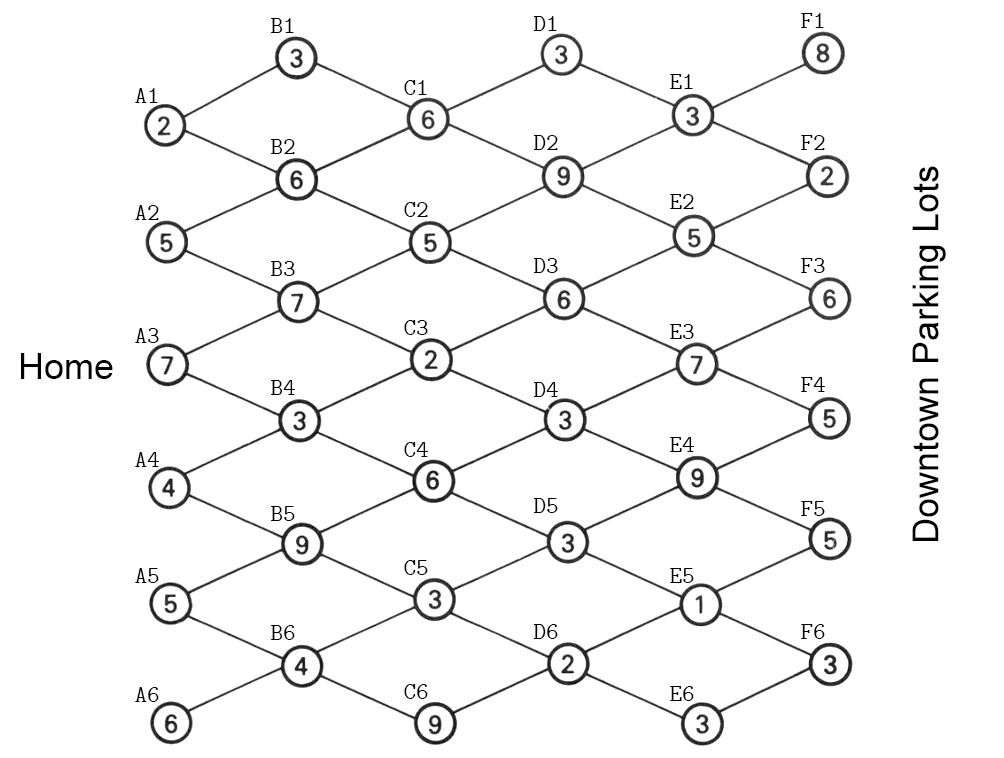
\includegraphics[width=0.9\linewidth]{parking.png}
    \caption{Path Network}
    \label{fig:net}
\end{figure}


\newpage

The problem can be formulated as a dynamic decision process with multiple stages, where the six columns of neighborhoods represent the six stages, with the following notations:

\begin{itemize}[nosep]
    \item \textbf{Stage} $t\in\{1,2,\dots,6\}$ represents the column in the network, where $T=6$ is the terminal stage
    \item \textbf{State} $s_t$, with $s_T$ as the terminal state and 
    \item \textbf{Action} $a(s_t)$, e.g. $a(s_t=\texttt{A3})=\texttt{B3}$
    \item \textbf{Transition Set} $N(s_t)$ is a set of all feasible next states that can be reached from the current state $s_t$
    \item \textbf{Cost Function} $g(s_t)$, e.g. $g(s_t=\texttt{B3})=7$
    \item \textbf{Cost-to-go Value} $J_t(s_t)$, with $J_T(s_T)$ for the terminal stage
\end{itemize}


\subsection{Written}

\begin{enumerate}[label=(\alph*)]

\item \grade{5} \sAll Which of the following statements are correct?
{
\checkboxchar{$\Box$} \checkedchar{$\blacksquare$}  % DO NOT CHANGE THIS LINE
\begin{checkboxes}
    \choice States refer to the specific node in the network at stages.
    \choice Actions refer to the decision of which neighboring node to move to next.
    \choice The number of states depends on the path chosen.
    \choice The cost function measures the travel time.
    \choice The cost-to-go value is the minimal travel time spent from home to the current state.
\end{checkboxes}
}


\item \grade{5} \sAll Which of the following statements are correct?
{
\checkboxchar{$\Box$} \checkedchar{$\blacksquare$}  % DO NOT CHANGE THIS LINE
\begin{checkboxes}
    \choice The first step of BI is to assign cost-to-go values to the home node.
    \choice The first step of BI is to choose the parking lot with the lowest cost.
    \choice BI computes the cost of all possible paths in this network.
    \choice If two different paths have the same minimum total cost, BI considers either path as optimal.
    \choice An optimal path must contain optimal sub-paths.
\end{checkboxes}
}


\item \grade{5} \sAll Which of the following would affect the optimal path in this network?
{
\checkboxchar{$\Box$} \checkedchar{$\blacksquare$}  % DO NOT CHANGE THIS LINE
\begin{checkboxes}
    \choice Close one of the parking lots
    \choice Change travel time inside a single neighborhood
    \choice Increase travel time in every node by the same constant
    \choice Adding extra edges between neighborhoods
    \choice Rename the node IDs
\end{checkboxes}
}


\item \grade{5} \saq Write the cost-to-go function \textit{(Tip: formualte $J_t(s_t)$ and $J_T(s_T)$ separately)}.
\begin{answerBox}[height=1.6in]

\end{answerBox}


\item \grade{10} \sCal Compute the cost-to-go value for node \texttt{D4}, $J_4(s_4=\texttt{D4})$. 
\\Include the calculation steps from the terminal stage to stage 4.
What is the action $a(s_4=\texttt{D4})$?
\begin{answerBox}[height=6in]

\end{answerBox}


\item \grade{5} \saq What is the optimal path of actions? Use the node ID.
\begin{answerBox}[height=2in]

\end{answerBox}

\end{enumerate}




\newpage
\section{Hospital Surge Staffing via Q-Learning}
\label{sec:q2}

In this assignment, we will revisit the Hospital Surge Staffing problem discussed in the recitation. 

As the following questions are based on the solution notebook, please study the notebook carefully before answering. You can find all \texttt{function()} and \texttt{class} mentioned in the questions from the notebook.

For your convenience, the solution notebook, named as \texttt{D2A\_A2\_HospitalStaffing.ipynb}, is included in the handout package. It is the recitation solution notebook posted on Canvas, with an added SARSA section at the end.

\subsection{Written}

\begin{enumerate}[label=(\alph*)]

\item \grade{5} \sAll Which of the following statements about the Q-learning update rule (Equation~\ref{eq:ql}) are correct?
\begin{equation}
    Q_t(x_t, u_t) \leftarrow (1-\alpha) Q_t(x_t,u_t) + \alpha \Bigl( r_t + \gamma \min_{u_{t+1}} Q_{t+1}(x_{t+1}, u_{t+1}) \Bigr)
    \label{eq:ql}
\end{equation}
{
\checkboxchar{$\Box$} \checkedchar{$\blacksquare$}  % DO NOT CHANGE THIS LINE
\begin{checkboxes}
    \choice It blends old and new estimates using the learning rate $\alpha$.
    \choice It uses the immediate cost plus the discounted best estimate of future cost.
    \choice It requires the full transition model of the environment to run.
    \choice It is a sample-based approximation of the Bellman optimality equation.
    \choice It ignores rewards or costs when updating.
\end{checkboxes}
}


\item \grade{5} \sAll Which of the following statements correctly describe the role of $\epsilon$-greedy exploration in Q-learning, i.e., the \texttt{choose\_action()} function of \texttt{QLearningAgent}?
{
\checkboxchar{$\Box$} \checkedchar{$\blacksquare$}  % DO NOT CHANGE THIS LINE
\begin{checkboxes}
    \choice It prevents the agent from prematurely converging to a suboptimal policy.
    \choice It guarantees the agent always finds the globally optimal solution.
    \choice It encourages trying actions with uncertain or unexplored values.
    \choice It balances the trade-off between learning new information and exploiting known information.
    \choice The agent will still explore sufficiently after removing $\epsilon$-greedy, because the learning rate $\alpha$ provides randomness.
\end{checkboxes}
}


\item \grade{5} \sAll Which of the following statements distinguish Backward Induction from Q-learning?
{
\checkboxchar{$\Box$} \checkedchar{$\blacksquare$}  % DO NOT CHANGE THIS LINE
\begin{checkboxes}
    \choice Backward induction requires full knowledge of the transition probabilities and costs.
    \choice Backward induction computes the exact cost-to-go function, while Q-learning estimates it iteratively.
    \choice Backward induction always converges faster than Q-learning, regardless of problem size.
    \choice Q-learning learns optimal policies through simulated or real experience.
    \choice Q-learning cannot achieve the optimal policy even with infinite training.
\end{checkboxes}
}


\item \grade{2} \saq When calling the \texttt{step()} function of \texttt{HospitalEnvQL}, one of the results is variable of next state. What does this next state variable include? Explain in words what it/they means/mean in the context of hospital surge staffing.
\begin{answerBox}[height=2in]

\end{answerBox}


\end{enumerate}


\vspace{1em}
\paragraph{Q-table} is one of the keys in tabular Q-learning. In the notebook, \texttt{QLearningAgent} initializes the Q-table using the code below, which is a 3-dimensional table. 

\begin{lstlisting}
        self.Q = np.zeros((T+2, X_MAX+1, U_MAX+1), dtype=float)
\end{lstlisting}

\begin{enumerate}[label=(\alph*), resume]

\item \grade{2} \saq What does each dimension represent in the context of hospital surge staffing?
\begin{answerBox}[height=2in]

\end{answerBox}


\item \grade{2} \saq Why is it \texttt{X\_MAX+1} instead of \texttt{X\_MAX} directly?
\begin{answerBox}[height=2in]

\end{answerBox}



\end{enumerate}


\newpage
\paragraph{Learning rates decay} over the course of learning in the notebook implementation. Therefore, we should formally write the update rule as Equation~\ref{eq:td} where $a_t$ varies over time.

\begin{equation}
    Q_t(x_t, u_t) \leftarrow (1-\alpha_t) Q_t(x_t,u_t) + \alpha_t \Bigl( r_t + \gamma \min_{u_{t+1}} Q_{t+1}(x_{t+1}, u_{t+1}) \Bigr) \label{eq:td}
\end{equation}

\begin{enumerate}[label=(\alph*), resume]

\item \grade{2} \sCode Which line of the \texttt{learn()} function of \texttt{QLearningAgent} in the notebook controls the learning rate decaying?
\begin{codeBox}[height=1.5in]

\end{codeBox}


\item \grade{5} \sAll Which of the following statements are correct?
{
\checkboxchar{$\Box$} \checkedchar{$\blacksquare$}  % DO NOT CHANGE THIS LINE
\begin{checkboxes}
    \choice A high learning rate $\alpha$ always guarantees faster and more stable convergence.
    \choice Decaying the learning rate $\alpha$ over time helps stabilize learning once Q-values are close to convergence.
    \choice The discount factor $\gamma$ controls how much future costs are taken into account relative to immediate ones.
    \choice If $\gamma=1$, future costs are considered equally important as immediate costs.
    \choice If both $\gamma$ and $\alpha$ are set to zero, Q-learning still converges to the optimal policy.
\end{checkboxes}
}


\item \grade{2} \saq The current $a_t$ follows a time-dependent linear decay until it reaches a minimum threshold. How would you modify this schedule to use a non-linear decay instead? \textbf{Express your answer as a formula of the form} $a_t = \dots$. Your proposed schedule could be either time-dependent or time-independent.
\begin{answerBox}[height=3in]
    
\end{answerBox}



\end{enumerate}


\paragraph{SARSA} (State-Action-Reward-State-Action) is a simpler reinforcement learning algorithm than Q-learning. The agent works similarly to Q-learning that takes actions, receives feedback, and continuously updates its behavior to maximize long-term rewards. 

SARSA updates the Q-value using Equation~\ref{eq:sarsa}. 

\begin{equation}
    Q_t(x_t, u_t) \leftarrow (1-\alpha_t) Q_t(x_t,u_t) + \alpha_t \Bigl( r_t + \gamma Q_{t+1}(x_{t+1}, u_{t+1})\Bigr)
    \label{eq:sarsa}
\end{equation}

As you can see, the key difference is that SARSA does not include $\min$ operation. Therefore, SARSA is an \textbf{on-policy} algorithm learning the value of the policy it is actually following, while Q-learning is \textbf{off-policy} that learns the value of the optimal policy while possibly following a different exploratory policy when taking actions.


\begin{enumerate}[label=(\alph*), resume]

\item \grade{3} \sAll Which of the algorithms eventually converge to the same Q-values, despite differences in the number of steps required for convergence?
{
\checkboxchar{$\Box$} \checkedchar{$\blacksquare$}  % DO NOT CHANGE THIS LINE
\begin{checkboxes}
    \choice Q-learning with $\epsilon$-greedy, where $\epsilon = 0.1$
    \choice SARSA with the same $\epsilon$-greedy, $\epsilon = 0.1$
    \choice SARSA with dynamic $\epsilon$-greedy, where $\epsilon$ is gradually reduced from 0.1 to 0
    \choice All three algorithms above lead to different Q-values
\end{checkboxes}
}


\item \grade{2} \saq Reason your answer to the above question.
\begin{answerBox}[height=4in]
    
\end{answerBox}


\end{enumerate}



\newpage
\section{Ride-hailing Pricing via Decision‑Dependent Predict-then-Optimize}
\label{sec:q3}

\subsection{Programming}

Complete the provided start Jupyter notebook, \texttt{D2A\_A2\_SurgePricing.ipynb}.

Export the following spreadsheets of your model results as guided in the notebook.

\begin{enumerate}[label=(\alph*)]
    \item \grade{10} \texttt{prediction\_test.csv}
    \item \grade{15} \texttt{optimization\_decisions.csv}
\end{enumerate}


\subsection{Written}

\begin{figure}[h!]
    \centering
    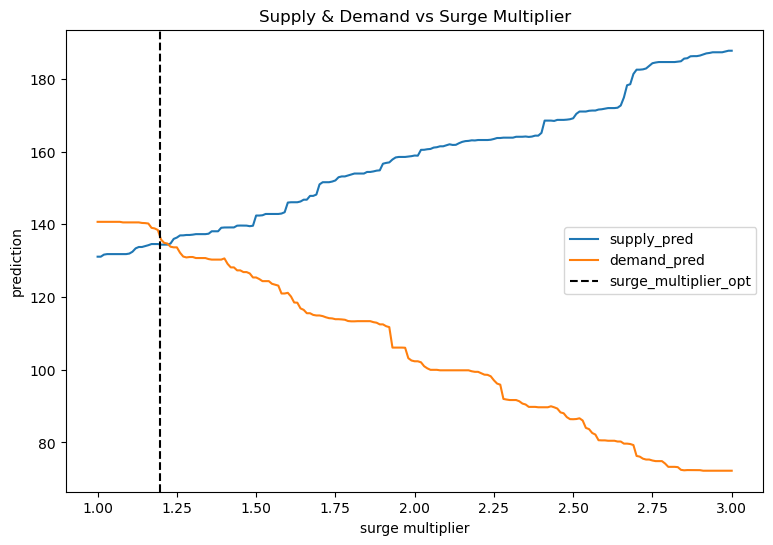
\includegraphics[width=0.8\linewidth]{equilibrium.png}
    \caption{Sample Plot of the Last Cell of the Notebook}
    \label{fig:equilibrium}
\end{figure}


\begin{enumerate}[label=(\alph*)]

\item \grade{3} \saq If your notebook is implemented correctly, the last cell should output a figure similar to Figure~\ref{fig:equilibrium}. The figure includes the supply and demand curves. The black dashed vertical line indicates where the optimized surge multiplier is. 
\\Carefully read the code and understand the plot. How do you interpret this plot?
\\(Answer box is on the next page)

\newpage
\begin{answerBox}[height=6in]
    
\end{answerBox}

\end{enumerate}

\vspace{1em}
\section*{Deliverables}
Congratulations! All of the work is complete. The last step is to submit your deliverables to Gradescope:

\begin{itemize}
    \item 1 single PDF file to ``\textbf{Assignment 2 Written}''
    \item the follwoing files to ``\textbf{Assignment 2 Programming}''
    \begin{itemize}
        \item \texttt{D2A\_A2\_SurgePricing.ipynb}
        \item \texttt{prediction\_test.csv}
        \item \texttt{optimization\_decisions.csv}
    \end{itemize}
\end{itemize}

\end{document}
